% =====================================================================
% Methodology Overview — Deep Learning Models of Loan Portfolios
% Standalone explainer: design rationale for the analysis & modelling plan.
% Compile: latexmk -pdf methodology_overview.tex   (or pdflatex x2)
% Cross-references: figure/table codes (T1.1, F3.4, ...) and tasks (M1-M15,
% MD1-MD4) refer to dev/model_plan/01_EDA.md, 02_LOAN_LEVEL.md,
% 03_POOL_LEVEL.md, 04_TASKS.md, 05_MACRO_DATA.md in the repository.
% =====================================================================
\documentclass[11pt,a4paper]{article}

\usepackage[margin=2.6cm]{geometry}
\usepackage{amsmath, amssymb, amsthm}
\usepackage{booktabs}
\usepackage{microtype}
\usepackage{enumitem}
\usepackage[font=small,labelfont=bf]{caption}
\usepackage[round]{natbib}
\usepackage{tikz}
\usetikzlibrary{positioning, arrows.meta}
\usepackage[colorlinks=true, linkcolor=blue!50!black, citecolor=blue!50!black, urlcolor=blue!50!black]{hyperref}

\newtheorem{remark}{Remark}
\newcommand{\E}{\mathbb{E}}
\newcommand{\Prob}{\mathbb{P}}
\newcommand{\R}{\mathbb{R}}
\newcommand{\code}[1]{\texttt{#1}}
\newcommand{\state}[1]{\textsf{#1}}
% artifact codes (tables/figures produced by the plan)
\newcommand{\artifact}[1]{\textbf{[#1]}}

\title{Modelling Mortgage State Transitions with Deep Learning:\\
\large A Methodological Overview of the Analysis Design\\
\normalsize (companion document to the \code{dev/model\_plan} specification)}
\author{Felipe Fritsch\\ \small MSc Mathematical \& Computational Finance, University of Oxford}
\date{June 2026}

\begin{document}
\maketitle

\begin{abstract}
\noindent This document explains, in a self-contained and didactic way, how the empirical analysis of the dissertation is designed and \emph{why} each design choice was made. The project replicates the framework of \citet{sirignano2021} on the Fannie Mae Single-Family Loan Performance dataset: a monthly state-transition model of mortgage behaviour estimated with deep neural networks and benchmarked against an empirical transition matrix and multinomial logistic regression, first at the loan level and then aggregated to pools. Throughout, bracketed codes such as \artifact{F3.4} or \artifact{Table B} refer to concrete figures and tables produced by the analysis pipeline, and codes M1--M15 / MD1--MD4 refer to the sequenced implementation tasks; Appendix~\ref{app:artifacts} provides the full map. The document is written to serve three purposes: my own consolidated understanding, discussions with my supervisor, and a quarry of prose for the dissertation itself.
\end{abstract}

\tableofcontents

% =====================================================================
\section{The research question and the modelling object}\label{sec:object}

A mortgage is a small dynamical system. In any month it occupies one of a small number of \emph{states} --- it is current, or 30/60/90+ days past due (DPD), or it has terminated through prepayment or a credit event --- and between consecutive months it moves between these states with probabilities that depend on the loan's characteristics and the economic environment. The cashflows of any mortgage portfolio or mortgage-backed security are completely determined by these movements: a prepayment returns principal early (a risk when rates have fallen), while the path $\state{current}\to\state{30}\to\state{60}\to\state{90+}\to\state{foreclosure}$ destroys value. Modelling the \emph{conditional transition distribution} is therefore the natural primitive for credit and prepayment risk.

Formally, let $S_{i,t}\in\mathcal{S}$ denote the state of loan $i$ in month $t$, and let $x_{i,t}\in\R^{d}$ collect everything observable about the loan and its environment at $t$ (its current state, static origination characteristics, dynamic loan fields, and macroeconomic covariates). The object of interest is
\begin{equation}
\label{eq:object}
p_\theta\!\left(j \mid x_{i,t}\right) \;\approx\; \Prob\!\left(S_{i,t+1}=j \,\middle|\, x_{i,t}\right), \qquad j\in\mathcal{S},
\end{equation}
a \emph{multinomial classification of next month's state}. Every model in this dissertation --- from a frequency-count matrix to an ensemble of deep networks --- is an estimator of \eqref{eq:object}; they differ only in how flexibly they let the probabilities depend on $x$.

The central empirical claim of \citet{sirignano2021}, which this dissertation tests on a different and cleaner dataset, is that the dependence of \eqref{eq:object} on $x$ is strongly \emph{nonlinear} and features economically meaningful \emph{interactions} between covariates (their flagship example: the prepayment response to a refinancing incentive depends on credit score and loan size). Linear models misspecify this dependence, and the misspecification compounds when loan-level probabilities are aggregated to pool-level cashflows --- the level at which securities are priced. The analysis is therefore organised as a horse race with three escalating phases:
\begin{enumerate}[itemsep=1pt]
  \item \textbf{Phase 1 (EDA, tasks M1--M3):} establish the dataset's scope and produce \emph{model-free} evidence of nonlinearity that motivates everything downstream (Section~\ref{sec:eda});
  \item \textbf{Phase 2 (loan-level models, M4--M12):} estimate \eqref{eq:object} with benchmarks of increasing flexibility --- empirical matrix, multinomial logit, deep networks, ensembles --- under a rolling out-of-sample design (Sections~\ref{sec:design}--\ref{sec:eval});
  \item \textbf{Phase 3 (pool-level analysis, M13--M15):} compose the monthly model into 12-month horizon predictions and compare models where it matters economically: predicted versus realised prepayment and delinquency counts in pools (Section~\ref{sec:pool}).
\end{enumerate}

% =====================================================================
\section{Data: the Fannie Mae loan-performance panel}\label{sec:data}

\subsection{What one row is, and why the data is 800\,GB}

The raw data are $\sim$100 quarterly CSV files totalling $\sim$800\,GB, published by Fannie Mae. Three different things in this dataset are all colloquially called a ``quarter,'' and distinguishing them prevents the most common assembly errors:
\begin{itemize}[itemsep=1pt]
  \item the \textbf{acquisition vintage} identifies a \emph{file}: each \code{YYYYQn.csv} contains the loans Fannie Mae acquired in that quarter, carrying their entire subsequent monthly history. A loan appears in exactly one file, so concatenating all files assembles the full sample with no duplication;
  \item the \textbf{monthly reporting period} identifies a \emph{row}: one row per loan per month. A surviving 30-year loan contributes up to $\sim$360 rows --- this time dimension, not redundancy, is why the dataset is large;
  \item the \textbf{release} identifies the \emph{download}: Fannie Mae republishes the entire dataset quarterly with extended histories. All files must come from one release, otherwise vintages have inconsistent right-censoring dates (the ingestion pipeline's Stage~1 audit verifies this).
\end{itemize}

The dataset covers vintages 2000Q1--2025 and is a deliberately clean credit box: 30-year fixed-rate, fully amortising, fully documented conventional loans with LTV $\le 97$. It excludes ARMs, subprime, interest-only and government-insured loans --- a stated contrast with the private-label data of \citet{sirignano2021} and a reason to expect lower delinquency base rates here.

\subsection{The data-engineering layer in one paragraph}

No single file fits in memory, so a six-stage pipeline (built and verified before this analysis began) converts the CSVs into a compressed, columnar \emph{Parquet} lake queried out-of-core by DuckDB: an integrity audit (Stage 1), streaming CSV$\to$Parquet conversion (2), type/sentinel cleaning (3), construction of the transition panel with the target variable (4), sampling and view helpers (5), and reconciliation QA (6). Two properties of this layer matter for the analysis. First, \emph{columnar storage} means a query touching 6 of the 113 columns reads roughly 5\% of the bytes, which is what makes repeated full-panel aggregations (the EDA, the empirical transition matrices) cheap. Second, the panel carries purpose-built \emph{derived columns} --- integer calendar keys \code{period\_ym}/\code{orig\_ym} for temporal masking, and a \code{shard} key for randomisation --- that encode the statistical discipline of Sections~\ref{sec:shards} and \ref{sec:design} directly in the data layout, so no downstream code can easily violate it.

% =====================================================================
\section{The state space and the supervised target}\label{sec:states}

\subsection{Seven states from two raw fields}

Each loan-month is assigned a state from
\[
\mathcal{S}=\{\state{current},\, \state{dpd\_30},\, \state{dpd\_60},\, \state{dpd\_90plus},\, \state{foreclosure},\, \state{REO},\, \state{prepaid}\},
\]
derived from two raw fields. In ordinary months, the \emph{delinquency status} code maps directly (\code{00}$\to$\state{current}, \code{01}$\to$\state{dpd\_30}, \code{02}$\to$\state{dpd\_60}, \code{03}+$\to$\state{dpd\_90plus}). In a loan's final month a \emph{zero-balance code} states how it terminated, mapping to \state{prepaid} (payoff, repurchase, non-credit removal) or to the credit-event terminals \state{foreclosure} (third-party/short/note sale, credit repurchase) and \state{REO}. The supervised label is the pair $(S_{i,t}, S_{i,t+1})$, with $S_{i,t+1}$ obtained by a per-loan window function; a loan's last observed month before the data cut-off has no successor and is flagged \emph{censored} and excluded from all likelihoods.

\begin{remark}[A $4\times 7$, not $7\times 7$, matrix]\label{rem:4x7}
In this dataset the terminal states exist \emph{only} as zero-balance codes in a loan's final month: there is no ongoing ``in foreclosure'' monthly status as in the CoreLogic data of \citet{sirignano2021}. Origin states are therefore $\mathcal{S}_{\mathrm{org}}=\{\state{current}, \state{dpd\_30}, \state{dpd\_60}, \state{dpd\_90plus}\}$ while destinations span all seven: the transition matrix is $4\times 7$ and \state{prepaid}/\state{foreclosure}/\state{REO} are absorbing. This is a documented deviation from the paper, but a harmless one for the model comparison, since every competing model conditions on the same origin set.
\end{remark}

Some transitions are structurally (near-)impossible --- delinquency deepens at most one bucket per month, so $\state{current}\to\state{dpd\_60}$ cannot occur, while cures can jump down arbitrarily. Rather than hard-coding a mask, the models are left to learn these zeros, and the evaluation suite \emph{asserts} that predicted mass on impossible cells is negligible --- a useful internal consistency check on the whole pipeline.

The class structure is extremely imbalanced: $\state{current}\!\to\!\state{current}$ accounts for the overwhelming majority of the $\sim$billion usable transitions, while $\state{dpd\_90plus}\!\to\!\state{REO}$ events are vanishingly rare \artifact{T1.3, T2.1}. Section~\ref{sec:thinning} explains how training exploits this without biasing the estimated probabilities.

% =====================================================================
\section{Model-free evidence: the EDA programme}\label{sec:eda}

Before any model is fitted, Phase 1 builds the empirical case that nonlinear modelling is \emph{needed} --- using only counting, no estimation. The instrument is the \emph{empirical hazard curve}: bucket a covariate into equal-population bins and plot the realised one-month transition rate per bin. Three exhibits carry the argument:
\begin{itemize}[itemsep=1pt]
\item \textbf{Prepayment vs.\ loan age} \artifact{F3.1}: the classic ``seasoning hump'' --- prepayment hazard rises, peaks, and decays with age. No monotone (let alone linear) term can represent it.
\item \textbf{Prepayment vs.\ refinancing incentive} \artifact{F3.2}: an S-shaped response around zero --- borrowers barely react until the option is meaningfully in the money, then react strongly, then saturate. This is the paper's flagship nonlinearity.
\item \textbf{Delinquency vs.\ FICO$\times$LTV} \artifact{F3.4}: a two-dimensional rate heatmap. If the FICO gradient steepens as LTV rises --- and it does --- the effects \emph{interact}, and no additive-linear model is correctly specified regardless of how its single-variable terms are transformed. This single figure is the most persuasive motivation exhibit in the dissertation.
\end{itemize}
Supporting exhibits map the terrain: transition rates over calendar time \artifact{F2.2} display the 2003 and 2020--21 refinancing waves, the 2008--11 default wave and the 2022--23 prepayment collapse (and double as a sanity check that the state derivation of Section~\ref{sec:states} is correct); vintage-cohort hazards \artifact{F3.6} isolate the notorious 2006--07 originations; and a COVID-era audit of delinquency codes \artifact{F2.3} documents how forbearance distorts 2020--21 records before models ever see them. Because each figure is a single out-of-core \code{GROUP BY} over the columnar panel, the entire programme runs in minutes --- a payoff of the engineering layer of Section~\ref{sec:data}.

% =====================================================================
\section{Randomisation at scale: shards}\label{sec:shards}

This section is deliberately didactic: sharding is the one piece of data engineering whose \emph{statistical} content is easy to miss, and it quietly underwrites both the SGD training loop and the integrity of the evaluation sets.

\subsection{The problem}

Stochastic gradient descent assumes minibatches are (approximately) random draws from the training distribution. The panel, however, is stored grouped by acquisition vintage --- reading it sequentially yields batches composed entirely of, say, 2007-vintage loans, whose risk profile is wildly atypical. Gradients computed on such batches are biased in a way that changes \emph{within} an epoch, and training quality degrades. The textbook remedy --- globally shuffle the dataset each epoch --- is infeasible for $\sim$$10^9$ rows on external storage.

\subsection{The construction}

The pipeline assigns every row a \emph{shard},
\begin{equation}
\label{eq:shard}
\code{shard}(i) \;=\; h\!\left(\code{LoanID}_i\right) \bmod N, \qquad N=256,
\end{equation}
where $h$ is a fixed-seed 64-bit hash function. Three properties follow, each load-bearing:

\begin{enumerate}[itemsep=2pt]
\item \textbf{Pseudo-random partition of \emph{loans}.} A good hash behaves like an independent uniform draw over $\{0,\dots,N-1\}$ \emph{per loan ID}; each shard is therefore an unbiased $\tfrac1N$ sample of loans, mixing all vintages, geographies and risk profiles \artifact{F5.1, F5.2}.
\item \textbf{Loan-disjointness.} Because the hash is keyed on the loan identifier --- not the row --- \emph{every} monthly observation of a loan lands in the same shard. A loan can never straddle two shards, which is what makes shard-based subsets safe for evaluation (Section~\ref{sec:design}): had the key been the row, ``20\% of loans'' would silently become ``20\% of every loan's rows,'' and held-out loans would also appear in training.
\item \textbf{Reproducibility without state.} The assignment is a pure function of the loan ID: rebuilding the panel, or ingesting a re-released vintage, reproduces every shard exactly, with no random seed to persist.
\end{enumerate}

The panel is physically \emph{sorted} by (\code{shard}, loan, month), so Parquet row-group statistics let the query engine skip directly to \code{WHERE shard = k} without scanning the lake --- one shard ($\sim$3--5M rows) is a cheap, RAM-sized read.

\subsection{The training loop it enables}

\begin{figure}[h]
\centering
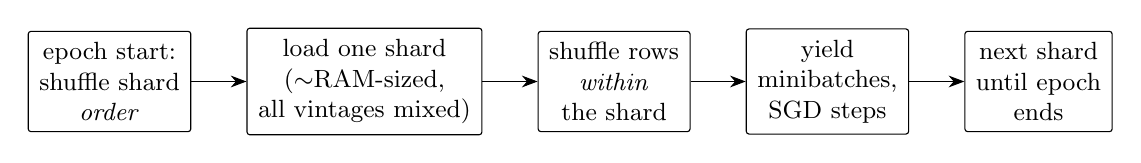
\begin{tikzpicture}[node distance=4mm and 7mm,
  box/.style={draw, rounded corners=1pt, align=center, font=\small, inner sep=4pt},
  arr/.style={-{Stealth[length=2mm]}}]
\node[box] (a) {epoch start:\\ shuffle shard\\ \emph{order}};
\node[box, right=of a] (b) {load one shard\\ ($\sim$RAM-sized,\\ all vintages mixed)};
\node[box, right=of b] (c) {shuffle rows\\ \emph{within}\\ the shard};
\node[box, right=of c] (d) {yield\\ minibatches,\\ SGD steps};
\node[box, right=of d] (e) {next shard\\ until epoch\\ ends};
\draw[arr] (a) -- (b);
\draw[arr] (b) -- (c);
\draw[arr] (c) -- (d);
\draw[arr] (d) -- (e);
\end{tikzpicture}
\caption{The two-level shuffle: random shard order across the epoch, full shuffle within each RAM-sized shard. Every minibatch mixes loans from all vintages at streaming cost; a global shuffle of $10^9$ rows is never performed.}
\label{fig:shardloop}
\end{figure}

The two-level shuffle of Figure~\ref{fig:shardloop} is the standard large-scale approximation to full shuffling: it is not \emph{exactly} a uniform draw (rows in the same batch share a shard), but because each shard is already an unbiased cross-section of loans, the residual within-shard correlation is negligible for gradient quality. This directly resolves the failure mode flagged in the early project notes --- ``if you load a subset from one quarter of data, the batch is biased.''

% =====================================================================
\section{Macroeconomic covariates}\label{sec:macro}

Loan-level fields alone cannot explain \emph{when} waves of prepayment and delinquency occur; the drivers are the rate environment, labour markets and house prices. Macro data enters the analysis as two tiny time-keyed tables (national: one row per month; state: one row per state-month) joined to loan-months \emph{at export time} --- the 800\,GB lake is never rewritten (tasks MD1--MD4).

\begin{table}[h]
\centering\small
\begin{tabular}{llllc}
\toprule
Variable & Source & Geography & Monthly value & Join lag \\
\midrule
\code{pmms30} (30y mortgage rate) & FRED \code{MORTGAGE30US} & national & month mean & 0\,m \\
\code{dgs10}, \code{slope\_10y2y} & FRED \code{DGS10}/\code{DGS2} & national & month mean & 0\,m \\
\code{unrate\_nat} & FRED \code{UNRATE} & national & as published & 1\,m \\
\code{unrate\_state} & FRED \code{\{POSTAL\}UR} & 50 states + DC & as published & 1\,m \\
\code{hpi} (house-price index) & Freddie Mac FMHPI & national + state & as published & 2\,m \\
\bottomrule
\end{tabular}
\caption{The macro covariate set. The \emph{join lag} encodes publication realism: a loan-month at calendar month $t$ is joined to the macro value of month $t-\ell$, since month-$t$ unemployment is only published in $t{+}1$ and the HPI roughly two months later. Using final-revision (rather than real-time) series is a stated limitation.}
\label{tab:macro}
\end{table}

Two engineered features carry most of the economic content:
\begin{align}
\label{eq:incentive}
\text{(refinancing incentive)} \qquad
\code{incentive}_{i,t} &= r^{\mathrm{cur}}_{i,t} - \code{pmms30}(t),\\[2pt]
\label{eq:mtmltv}
\text{(mark-to-market LTV)} \qquad
\code{ltv\_mtm}_{i,t} &= \frac{\mathrm{UPB}_{i,t}}{\mathrm{UPB}_{i,0}}\;\cdot\;\mathrm{LTV}_{i,0}\;\cdot\;\frac{H_{s(i)}\!\left(t_0(i)\right)}{H_{s(i)}(t)},
\end{align}
where $H_s(\cdot)$ is the state-$s$ HPI and $t_0(i)$ the origination month. Equation~\eqref{eq:incentive} is the canonical prepayment driver --- the option to refinance is in the money when the borrower's rate exceeds the market rate --- and the locus of the strongest nonlinearity in \citet{sirignano2021} (an S-shaped response around zero, \artifact{F3.2}). Equation~\eqref{eq:mtmltv} marks the borrower's leverage to market: the original LTV is scaled by amortisation ($\mathrm{UPB}_t/\mathrm{UPB}_0$) and by house-price growth since origination, approximating current equity --- the key default driver. State-level joins matter because the cross-sectional dispersion in unemployment and housing drawdowns (Nevada vs.\ Texas in 2009) is precisely the variation a national series cannot supply \artifact{F4.3}.

A small but instructive point: an earlier design derived a market-rate proxy \emph{from the panel itself} (the average note rate of newly originated loans each month). It tracks the PMMS closely \artifact{F4.1} and is retained as a robustness check --- a useful demonstration that the incentive variable is not an artefact of one data source. Raw calendar time, by contrast, is deliberately \emph{excluded} as a feature: test years are by construction unseen, so a model leaning on ``year'' would extrapolate arbitrarily; all time variation must flow through observable, recurring channels (macro variables, seasonality, loan age).

% =====================================================================
\section{Experimental design: rolling out-of-sample estimation}\label{sec:design}

\subsection{Why temporal splits, and why strict masks}

Credit models are used prospectively, so the only honest evaluation is temporal: train on the past, predict the future. Random row-level splits would be doubly wrong here --- they leak within-loan information across the split \emph{and} let the model see the future of the very cycle it is being tested on.

One subtlety deserves emphasis because it is a one-character bug with real leakage consequences. The label of the example built at feature month $t$ is the state at $t{+}1$. ``Training on data up to month $T$'' must therefore mask on the \emph{label} month: include the example only if $t < T$ (strict), so that its label month $t{+}1 \le T$. Masking with $t\le T$ would include examples whose labels lie at $T{+}1$ --- one month of future information. The panel's integer calendar key makes this a one-line filter, \code{period\_ym < cutoff}.

\subsection{The rolling expanding-window backtest}

The primary design is a \emph{rolling, expanding-window backtest} with one window per test year $k = 2015,\dots,2025$:
\[
\underbrace{\text{train: labels} \le \mathrm{Dec}(k{-}2)}_{\text{expanding, starts 2000}}
\qquad
\underbrace{\text{validation: labels in year } k{-}1}_{\text{early stopping only}}
\qquad
\underbrace{\text{test: labels in year } k}_{\text{never touched in fitting}}
\]
so the first window trains through 2013, early-stops on 2014, and predicts 2015; the last predicts 2025. Three design rules keep this honest and affordable:
\begin{enumerate}[itemsep=2pt]
\item \textbf{Tune once, freeze, roll (M9--M10).} Architecture and regularisation hyperparameters are selected \emph{once}, on the $k{=}2015$ ``tuning window'' (with a spot-check on $k{=}2019$), then frozen across all windows; per-window validation sets serve only early stopping. Re-tuning every window would multiply compute by the grid size and constitute a subtle multiple-testing problem.
\item \textbf{Window-local preprocessing.} Feature scalers, embedding vocabularies and any statistic estimated from data are re-fitted within each window's training slice. Standardising with full-sample moments would leak future means and variances into the past.
\item \textbf{Pooled and per-year reporting.} Each test row in 2015--2025 is predicted exactly once, by a model that never saw it; metrics are reported per test year and pooled over all years \artifact{Table B}. Regime shifts --- COVID 2020--21, the 2022--23 rate spike --- thus appear as legible test-year effects rather than hinging on a single arbitrary cutoff.
\end{enumerate}

\subsection{Class thinning with importance weights}\label{sec:thinning}

Training on every $\state{current}\!\to\!\state{current}$ row is wasteful: they are $\sim$95\% of rows and individually nearly uninformative. The export therefore keeps every row whose origin or destination is \emph{not} \state{current}, but retains $\state{current}\!\to\!\state{current}$ rows only with probability $p$ (e.g.\ $p = 0.05$--$0.10$), attaching the weight $w_i = 1/p$ to kept rows (and $w_i=1$ otherwise). The training objective is the weighted negative log-likelihood
\begin{equation}
\label{eq:weightednll}
\widehat{\mathcal{L}}(\theta) \;=\; \frac{1}{\sum_i w_i}\sum_{i \in \text{kept}} w_i\,
\bigl[-\log p_\theta\!\left(y_i \mid x_i\right)\bigr],
\end{equation}
which is a Horvitz--Thompson estimator of the full-sample loss: since each row is kept with known probability $\pi_i \in \{p, 1\}$ and weighted by $1/\pi_i$, $\E[\widehat{\mathcal{L}}] $ equals the unthinned objective. The fitted model therefore still estimates the \emph{true} conditional probabilities --- unlike naive downsampling, which would silently inflate every rare-event probability by a factor of order $1/p$. Two guard-rails enforce this: validation and test slices are \emph{never} thinned, and the QA step compares ensemble-average predicted base rates against unthinned panel frequencies.

The evaluation pool is a fixed, loan-disjoint shard block (e.g.\ $\code{shard} < 0.2N$, i.e.\ $\sim$20\% of \emph{loans}, the same loans forever): large enough for tight metrics, small enough that scoring all $11$ windows $\times$ all models stays cheap, and identical across every model so that likelihood comparisons are exact, not sampled-apart.

% =====================================================================
\section{The model hierarchy}\label{sec:models}

The benchmarks are ordered by how flexibly they let \eqref{eq:object} depend on covariates; each strictly nests or dominates the previous in expressiveness, which is what makes the comparison interpretable.

\subsection{Model A: the empirical transition matrix}

The simplest estimator ignores covariates entirely: conditional only on the origin state $u$, estimate the destination distribution by smoothed relative frequencies in the window's training slice,
\begin{equation}
\label{eq:empirical}
\widehat{P}_{uv} \;=\; \frac{N_{uv} + \alpha}{N_{u\cdot} + \alpha\,|\mathcal{S}|}, \qquad \alpha = \tfrac12,
\end{equation}
where $N_{uv}$ counts $u\to v$ transitions. The Laplace term $\alpha$ guarantees no test transition receives probability zero (one unsmoothed empty cell would make the test log-likelihood $-\infty$). This is a time-homogeneous Markov chain --- the dumbest defensible model and the floor of the comparison \artifact{T2.1, Tables A/B}. A ``bucketed'' variant conditioning additionally on FICO and incentive terciles shows how far cheap, nonparametric conditioning goes before any model fitting.

\subsection{Model B: multinomial logistic regression --- a zero-layer network}

The workhorse of the empirical mortgage literature posits log-linear odds:
\begin{equation}
\label{eq:logit}
p_\theta(j \mid x) \;=\; \operatorname{softmax}_j\!\left(Wx + b\right)
\;=\; \frac{\exp\!\left(w_j^\top x + b_j\right)}{\sum_{j'} \exp\!\left(w_{j'}^\top x + b_{j'}\right)}.
\end{equation}
Crucially, \eqref{eq:logit} is exactly a neural network with \emph{zero hidden layers}, and it is implemented as such --- same data loader, same loss \eqref{eq:weightednll}, same evaluation code as the deep models, with a one-time numerical cross-check against \code{scikit-learn}. This is a deliberate experimental-control choice: when the deep network beats the logit, the difference is attributable to \emph{architecture alone}, not to differences in preprocessing, optimisation, or data. An ``augmented'' logit with hand-crafted nonlinear terms (squared loan age, splined incentive) quantifies how much of the gap manual feature engineering can close --- the traditional econometrician's rebuttal, given its fair hearing.

\subsection{Model C: deep neural networks}

The deep model composes $L$ hidden layers,
\begin{equation}
\label{eq:mlp}
z^{(0)} = \phi(x), \qquad
z^{(\ell)} = \sigma\!\left(W^{(\ell)} z^{(\ell-1)} + b^{(\ell)}\right), \qquad
p_\theta(\cdot \mid x) = \operatorname{softmax}\!\left(W^{(L+1)} z^{(L)} + b^{(L+1)}\right),
\end{equation}
with ReLU activations $\sigma(u)=\max(u,0)$ and the paper's preferred geometry (five hidden layers, 200 then $4\times140$ units) as the anchor of a depth grid $L\in\{1,3,5,7\}$. The input map $\phi$ standardises continuous features (window-local, per Section~\ref{sec:design}) and embeds categorical ones: high-cardinality fields like state, MSA and ZIP3 are mapped to learned dense vectors rather than one-hot columns, with unseen test levels routed to a reserved \code{UNK} embedding. Each hidden unit is a learned ``soft feature''; depth lets the network build feature hierarchies, which is precisely where interaction effects like incentive$\times$FICO live --- the model discovers \artifact{F3.5} rather than being told it.

\paragraph{Regularisation.} Three devices, mirroring the paper, with their selection documented in the tuning-window ablation \artifact{Table A}:
\begin{itemize}[itemsep=1pt]
\item \emph{Dropout}: randomly zeroing hidden units during training (rates $\{0, 0.2, 0.5\}$) prevents co-adaptation; the paper finds dropout shifts the optimal depth, a finding the grid replicates or refutes;
\item \emph{$\ell_2$ penalty} $\lambda\|\theta\|_2^2$, $\lambda\in\{0, 10^{-5}, 10^{-4}\}$;
\item \emph{Early stopping} on the window's validation NLL --- the only use the validation year is put to.
\end{itemize}

\paragraph{Ensembling.} The final model averages the predicted \emph{probabilities} of $K{=}8$ independently initialised networks trained on resampled shard subsets:
$\bar p(j\mid x) = \tfrac1K \sum_k p_{\theta_k}(j \mid x)$.
Averaging reduces the variance component of error from SGD randomness and finite data; the marginal value of each additional member is traced in the ensemble-size curve \artifact{F: ensemble curve, M9}. Because eight fits per window is the dominant compute cost, the ensemble runs on five regime-spanning key windows ($k\in\{2015, 2019, 2020, 2023, 2025\}$), with the single best network everywhere.

% =====================================================================
\section{Evaluation}\label{sec:eval}

\subsection{Likelihood as the headline metric}

The headline criterion is the out-of-sample mean negative log-likelihood,
\begin{equation}
\label{eq:nll}
\mathrm{NLL} \;=\; -\frac{1}{N_{\mathrm{test}}} \sum_{i\in\mathrm{test}} \log p_\theta\!\left(y_i \mid x_i\right),
\end{equation}
on \emph{identical, frozen, unthinned} test rows for every model. NLL is the right primary metric for this problem for two reasons: it evaluates the full predicted \emph{distribution} over seven destinations (not a binarised event), and it is a strictly proper scoring rule --- it is uniquely minimised in expectation by the true conditional probabilities, so a model cannot improve it by distorting its probabilities. Results are reported per test year and pooled \artifact{Table B}, by origin state (the gains should concentrate in \state{current} rows, i.e.\ prepayment behaviour), and in a tuning-window depth grid mirroring the paper's Table~11 \artifact{Table A}.

\subsection{Discrimination and calibration}

Two complementary lenses, because a single number hides failure modes:
\begin{itemize}[itemsep=1pt]
\item \emph{Discrimination} --- for each origin state $u$ and destination $v$, the one-vs-rest AUC: the probability that a randomly chosen loan-month that truly transitions $u\to v$ receives a higher predicted $p(v)$ than one that does not. AUC isolates \emph{ranking} quality, which is what matters for relative-value and screening uses \artifact{AUC table}.
\item \emph{Calibration} --- reliability diagrams for the major transitions ($\state{current}\to\state{prepaid}$, $\state{current}\to\state{dpd\_30}$): bucket predictions by predicted probability and compare to realised frequencies. A model can rank well yet be systematically over- or under-confident; calibration is what pool-level counting (Section~\ref{sec:pool}) actually consumes. A time-series overlay of predicted vs.\ realised aggregate transition rates over 2015--2025 doubles as the bridge exhibit to Phase 3.
\end{itemize}

\subsection{Robustness: is the comparison stable?}

Since the rolling backtest is itself the main design, robustness asks whether the model \emph{ranking} is an artefact: the depth/dropout ablation and ensemble curve (overfitting exhibits, \artifact{Table A}), seed variance of the best network against the NN--logit gap (is the edge larger than training noise?), ranking stability across the eleven test years (does the deep model's advantage survive COVID 2020--21 and the 2022--23 prepayment collapse, or only hold on average?), and a tuning-window sensitivity check (re-tuning on $k{=}2019$: does the same configuration win?).

% =====================================================================
\section{From loans to pools}\label{sec:pool}

\subsection{Why pool-level accuracy is the economic test}

A mortgage pool's cashflow is the sum of its loans' events; an MBS is priced off exactly such sums. Pool-level prediction is therefore where loan-level model differences either matter or wash out --- and \citet{sirignano2021} argue the nonlinearity advantage \emph{compounds} rather than washes out, because linear misspecification correlates across loans sharing characteristics. Phase 3 tests this with the frozen Phase-2 models; nothing is re-fitted.

\subsection{Multi-month prediction by matrix composition}

The monthly model is rolled forward by composing transition matrices. For loan $i$ alive at anchor month $t_0$ with state distribution $\rho_0$ (a one-hot vector), the model supplies, for each future month $h$, a $7\times 7$ matrix $P^{(i)}_h$ whose four non-terminal rows are the model's predictions at the (deterministically evolved) covariates and whose terminal rows are identity (absorbing). Then
\begin{equation}
\label{eq:rollforward}
\rho_h \;=\; \rho_0 \prod_{h'=1}^{h} P^{(i)}_{h'},
\qquad
\Prob\!\left(\text{loan } i \text{ prepaid by } t_0{+}H\right) = \left[\rho_H\right]_{\state{prepaid}},
\end{equation}
with $H=12$. Because terminal states are absorbing and the full state distribution is tracked, \eqref{eq:rollforward} is \emph{exact} under the model --- no Monte Carlo simulation is needed (the paper's simulation machinery exists for stochastic macro scenarios, which are out of scope; here covariates evolve deterministically --- age and remaining term advance, seasonality follows the calendar --- while UPB and the macro block are frozen at $t_0$, making predictions explicitly \emph{conditional on the anchor-date environment}).

For \emph{ever-delinquent} events (``reaches 60+ DPD within 12 months'') a first-passage construction is required: in the composed chain, delinquency states can be entered and \emph{cured out of}, so the month-12 occupancy of \state{dpd\_60} undercounts loans that visited and recovered. The fix is standard: build a modified chain $\widetilde P$ in which the target set is made absorbing; the absorbed mass at $H$ is then exactly the probability of \emph{ever} hitting the set by $H$.

\subsection{Pools, predictions, and the comparison}

Pools are formed two ways at each window anchor: \emph{characteristic buckets} (FICO $\times$ original rate $\times$ LTV cells, the criteria a structurer would use) and \emph{random pools} ($B{=}500$ pools of $N{=}1{,}000$ loans), which give a bucketing-free scatter. With per-loan horizon probabilities $q_i$ from \eqref{eq:rollforward}, the predicted event count in pool $\mathcal{P}$ and its distribution are
\begin{equation}
\label{eq:poolcount}
\widehat{C}_{\mathcal{P}} = \sum_{i\in\mathcal{P}} q_i,
\qquad
C_{\mathcal{P}} \;\dot\sim\; \mathcal{N}\!\Bigl(\textstyle\sum_i q_i,\; \sum_i q_i(1-q_i)\Bigr),
\end{equation}
the Gaussian being the standard approximation to the Poisson--binomial distribution of a sum of independent, non-identical Bernoullis (conditional independence given covariates is the maintained assumption, inherited from the paper). The comparison is then direct and visual: predicted vs.\ realised counts per pool \artifact{F4.1}, $R^2$/RMSE by model, outcome and anchor \artifact{T4.2} --- the relative RMSE reduction of the ensemble over the logit is the dissertation's headline economic number --- and signed errors across characteristic buckets \artifact{F4.3}, which localise \emph{where} the linear model breaks (the prediction: high-incentive cells). Interval coverage (the share of random pools whose realised count falls inside the model's 90\% band) tests \eqref{eq:poolcount}'s distributional claim, not just its mean.

% =====================================================================
\section{Reproducibility and operational discipline}\label{sec:repro}

Every model fit writes a self-describing run folder (configuration, git commit, data-manifest hash, window identity, metrics), so any number in the dissertation can be traced to the exact code and data slice that produced it. The implementation is sequenced as tasks M1--M15 with explicit acceptance criteria, executed one at a time with the evidence verified before advancing; correctness-critical components carry unit tests (the leakage mask, the importance weights, the \code{ltv\_mtm} formula, the roll-forward engine against a closed-form toy chain, and the $h{=}1$ consistency of Phase 3 against Phase 2's evaluator). Irreplaceable small artifacts (models, metrics, figures, manifests) are mirrored off the data drive at every milestone; the bulky lakes are deliberately \emph{not} backed up, being rebuildable from the immutable raw data.

% =====================================================================
\appendix
\section{Artifact and task cross-reference}\label{app:artifacts}

\begin{table}[h]
\centering\small
\begin{tabular}{lll}
\toprule
Code & Content & Produced by \\
\midrule
\artifact{T1.1--T1.3} & vintage coverage; covariate summary; state distribution by year & M1 \\
\artifact{T2.1, F2.2--F2.4} & pooled empirical matrix; transition rates over time; COVID codes; roll rates & M2 \\
\artifact{F3.1--F3.6} & hazard curves (age, incentive, FICO); FICO$\times$LTV and incentive$\times$FICO & M3 \\
 & interaction heatmaps; vintage effects & \\
\artifact{F4.1} & panel-derived market-rate proxy vs.\ PMMS & M3 \\
\artifact{F4.2--F4.3} & macro series small-multiples; state-dispersion exhibit & MD4 \\
\artifact{F5.1--F5.2} & shard balance and shard$\times$vintage mix checks & M3 \\
\artifact{Table A} & tuning-window depth/regularisation grid (paper's Table 11 analogue) & M9 \\
\artifact{Table B} & test-year $\times$ model NLL matrix + pooled all-years NLL & M10--M11 \\
\artifact{AUC table} & one-vs-rest AUC by origin and destination state & M11 \\
\artifact{Calibration} & reliability diagrams; predicted vs.\ realised rate overlay 2015--25 & M11 \\
\artifact{Pool F4.1, T4.2, F4.3} & predicted-vs-realised scatter; $R^2$/RMSE table; bucket error map & M14--M15 \\
\bottomrule
\end{tabular}
\caption{Map from artifact codes used in this document to the plan tasks that produce them. Task definitions and acceptance criteria: \code{dev/model\_plan/04\_TASKS.md}; EDA codes: \code{01\_EDA.md}; model/evaluation codes: \code{02\_LOAN\_LEVEL.md}; pool codes: \code{03\_POOL\_LEVEL.md}; macro: \code{05\_MACRO\_DATA.md}.}
\label{tab:artifactmap}
\end{table}

\section{Notation summary}\label{app:notation}

\begin{table}[h]
\centering\small
\begin{tabular}{ll}
\toprule
Symbol & Meaning \\
\midrule
$S_{i,t}\in\mathcal{S}$ & state of loan $i$ in month $t$; $|\mathcal{S}|=7$, origins $\mathcal{S}_{\mathrm{org}}$ (4 states) \\
$x_{i,t}\in\R^d$ & covariates: current state, loan fields, macro block, seasonality \\
$p_\theta(j\mid x)$ & model's one-month transition probability \eqref{eq:object} \\
$\code{period\_ym}, \code{orig\_ym}$ & integer calendar keys ($YYYYMM$) of reporting / origination month \\
$\code{shard} = h(\mathrm{ID}) \bmod 256$ & loan-keyed hash partition \eqref{eq:shard} \\
$k$; $T_k$ & backtest window / test year; its training cutoff $\mathrm{Dec}(k{-}2)$ \\
$w_i = 1/\pi_i$ & importance weight undoing class thinning \eqref{eq:weightednll} \\
$\widehat P_{uv}$ & Laplace-smoothed empirical transition matrix \eqref{eq:empirical} \\
$L$; $K$ & hidden-layer count \eqref{eq:mlp}; ensemble size ($K=8$) \\
$\rho_h$; $H$ & rolled-forward state distribution \eqref{eq:rollforward}; horizon ($H=12$) \\
$\widehat{C}_{\mathcal{P}}$, $q_i$ & predicted pool event count \eqref{eq:poolcount}; per-loan horizon probability \\
\bottomrule
\end{tabular}
\caption{Notation used throughout.}
\end{table}

% =====================================================================
\begin{thebibliography}{9}

\bibitem[Sirignano et~al.(2021)Sirignano, Sadhwani, and Giesecke]{sirignano2021}
Sirignano, J., Sadhwani, A., \& Giesecke, K. (2021).
\newblock Deep Learning for Mortgage Risk.
\newblock \emph{Journal of Financial Econometrics}, 19(2), 313--368.

\bibitem[Srivastava et al.(2014)]{dropout}
Srivastava, N., Hinton, G., Krizhevsky, A., Sutskever, I., \& Salakhutdinov, R. (2014).
\newblock Dropout: A Simple Way to Prevent Neural Networks from Overfitting.
\newblock \emph{Journal of Machine Learning Research}, 15, 1929--1958.

\bibitem[Goodfellow et al.(2016)]{goodfellow}
Goodfellow, I., Bengio, Y., \& Courville, A. (2016).
\newblock \emph{Deep Learning}. MIT Press.

\bibitem[Horvitz \& Thompson(1952)]{ht1952}
Horvitz, D.~G., \& Thompson, D.~J. (1952).
\newblock A Generalization of Sampling Without Replacement from a Finite Universe.
\newblock \emph{Journal of the American Statistical Association}, 47(260), 663--685.

\end{thebibliography}

\end{document}
